\section{Depth cameras' working principles}

The world of computer vision has, in recent years, benefit a lot of new hardware
technologies and improvement. In particular, object pose estimation algorithms
have been developed which, differently from the past ones which based themselves
either on standard, RGB images, or on couples of RGB images to use for
stereoscopic vision, exploit new generations of camera sensors which can provide
3D data to the user. Within the most common types of these are comprehended the
so-called \emph{depth sensors}; these particular kinds of sensors can provide
the user with an image which is built of floating-point, or integer, values,
each representing the distance from the sensor itself to the nearest obstacle
within line-of-sight, along the sensor's axis. If combined with the commonly
used geometric model for a camera, described in detail in sec.
\ref{sec:camera_modelling}, this measurement can lead to having not only a $z$
coordinate for each sampled point, but a complete 3D point $P=(x,y,z)$.

Other known approaches have been used in the past to obtain 3D vision systems:
in particular, the stereoscopic (or \emph{binocular}) system -- i.e., emulating the human vision by usage
of two different cameras -- has been widely studied and used, particularly into
the robotics' field, leading to
results such as \cite{stereo-vision-robot}; using this system, images taken
from two cameras are first scanned for correspondent, influential features
(\emph{keypoints}); pose information for each keypoint is then extracted from
the geometrical properties of the system in what is called \emph{triangulation}
as shown in fig. \ref{fig:stereo-triangulate}.

\begin{figure}[htbp]
\centering
\includegraphics[width=3in]{./Graphics/stereo-triangulate}
\caption{Two different cameras can match the same feature into different points
of their image: these will allow to extract 3D coordinates for the feature.\label{fig:stereo-triangulate}}
\end{figure}

Anyway, this approach has several limitations and can't be applied for proper
pose estimation of objects. Advantages of using depth sensors instead of
stereoscopic cameras include:
\begin{itemize}
  \item{Stereoscopic cameras can't produce an image with depth information for
      each pixel: in fact, this system is optimised for measuring depth over a
      small subset of the image (the keypoints), while completely ignoring the
      rest of the pixels. This comes as a natural consequence of the fact that
      features must be matched together in order to produce a depth information,
    as points in the background will seldom own such features;}
  \item{Although the previous problem could be solved by only looking for
      objects' keypoints when recognizing them, stereoscopic vision also can't
      be, by nature, as precise as depth sensors; \cite{stereo-precision} has
      shown that in order to have $2\unit{mm}$ of error in depth measurements
      with these systems, one must have precise information about the
      geometrical properties of the searched object, and must apply strong data
      filters in order not to have a high number of outliers; on the other hand,
      good depth sensors such as Occipital's Structure have an average error of
    some fractions of millimetre;}
  \item{Searching for matches into images in order to obtain good precision in
      stereoscopic vision is computationally expensive; also, effectiveness of
      these algorithms suffers from common RGB vision problems such as
    illumination changes or weakly textured images.}
\end{itemize}

Obviously, depth sensors have their disadvantages too: the most problematic one
is usually their very limited range of operation. For example, Microsoft
Kinect's Primesense module can sense in a range going from about $80\unit{cm}$
to about $3\unit{m}$; this makes it useless to adopt a visual depth sensor as
the main vision system in large environments, while stereoscopic vision,
especially if implemented with a high-definition camera, has
virtually no limit (except for focal loss) to the maximum depth it can sense;
this is the main reason for which stereoscopic vision is preferred for
autonomous robots, smart-cities, or search-and-rescue applications. Anyway, this
limited range is adequate for gripping purposes, as the objects will ordinarily
stand fixed within a range of one to two metres from the robotic arm.

For this project, two different type of depth cameras have been used: the first
is Microsoft Kinect, a common camera which can merge together both depth and RGB
informations, widely used in both consumer and research environment,
the layout of which is shown in fig. \ref{fig:kinect}; the second is Occipital's
Structure sensor, which is a depth-only camera with optimal minimum range
($40\unit{cm}$) and precision capabilities (about $1\unit{mm}$ of maximum error,
with very reduced noise).

\begin{figure}[htbp]
\centering
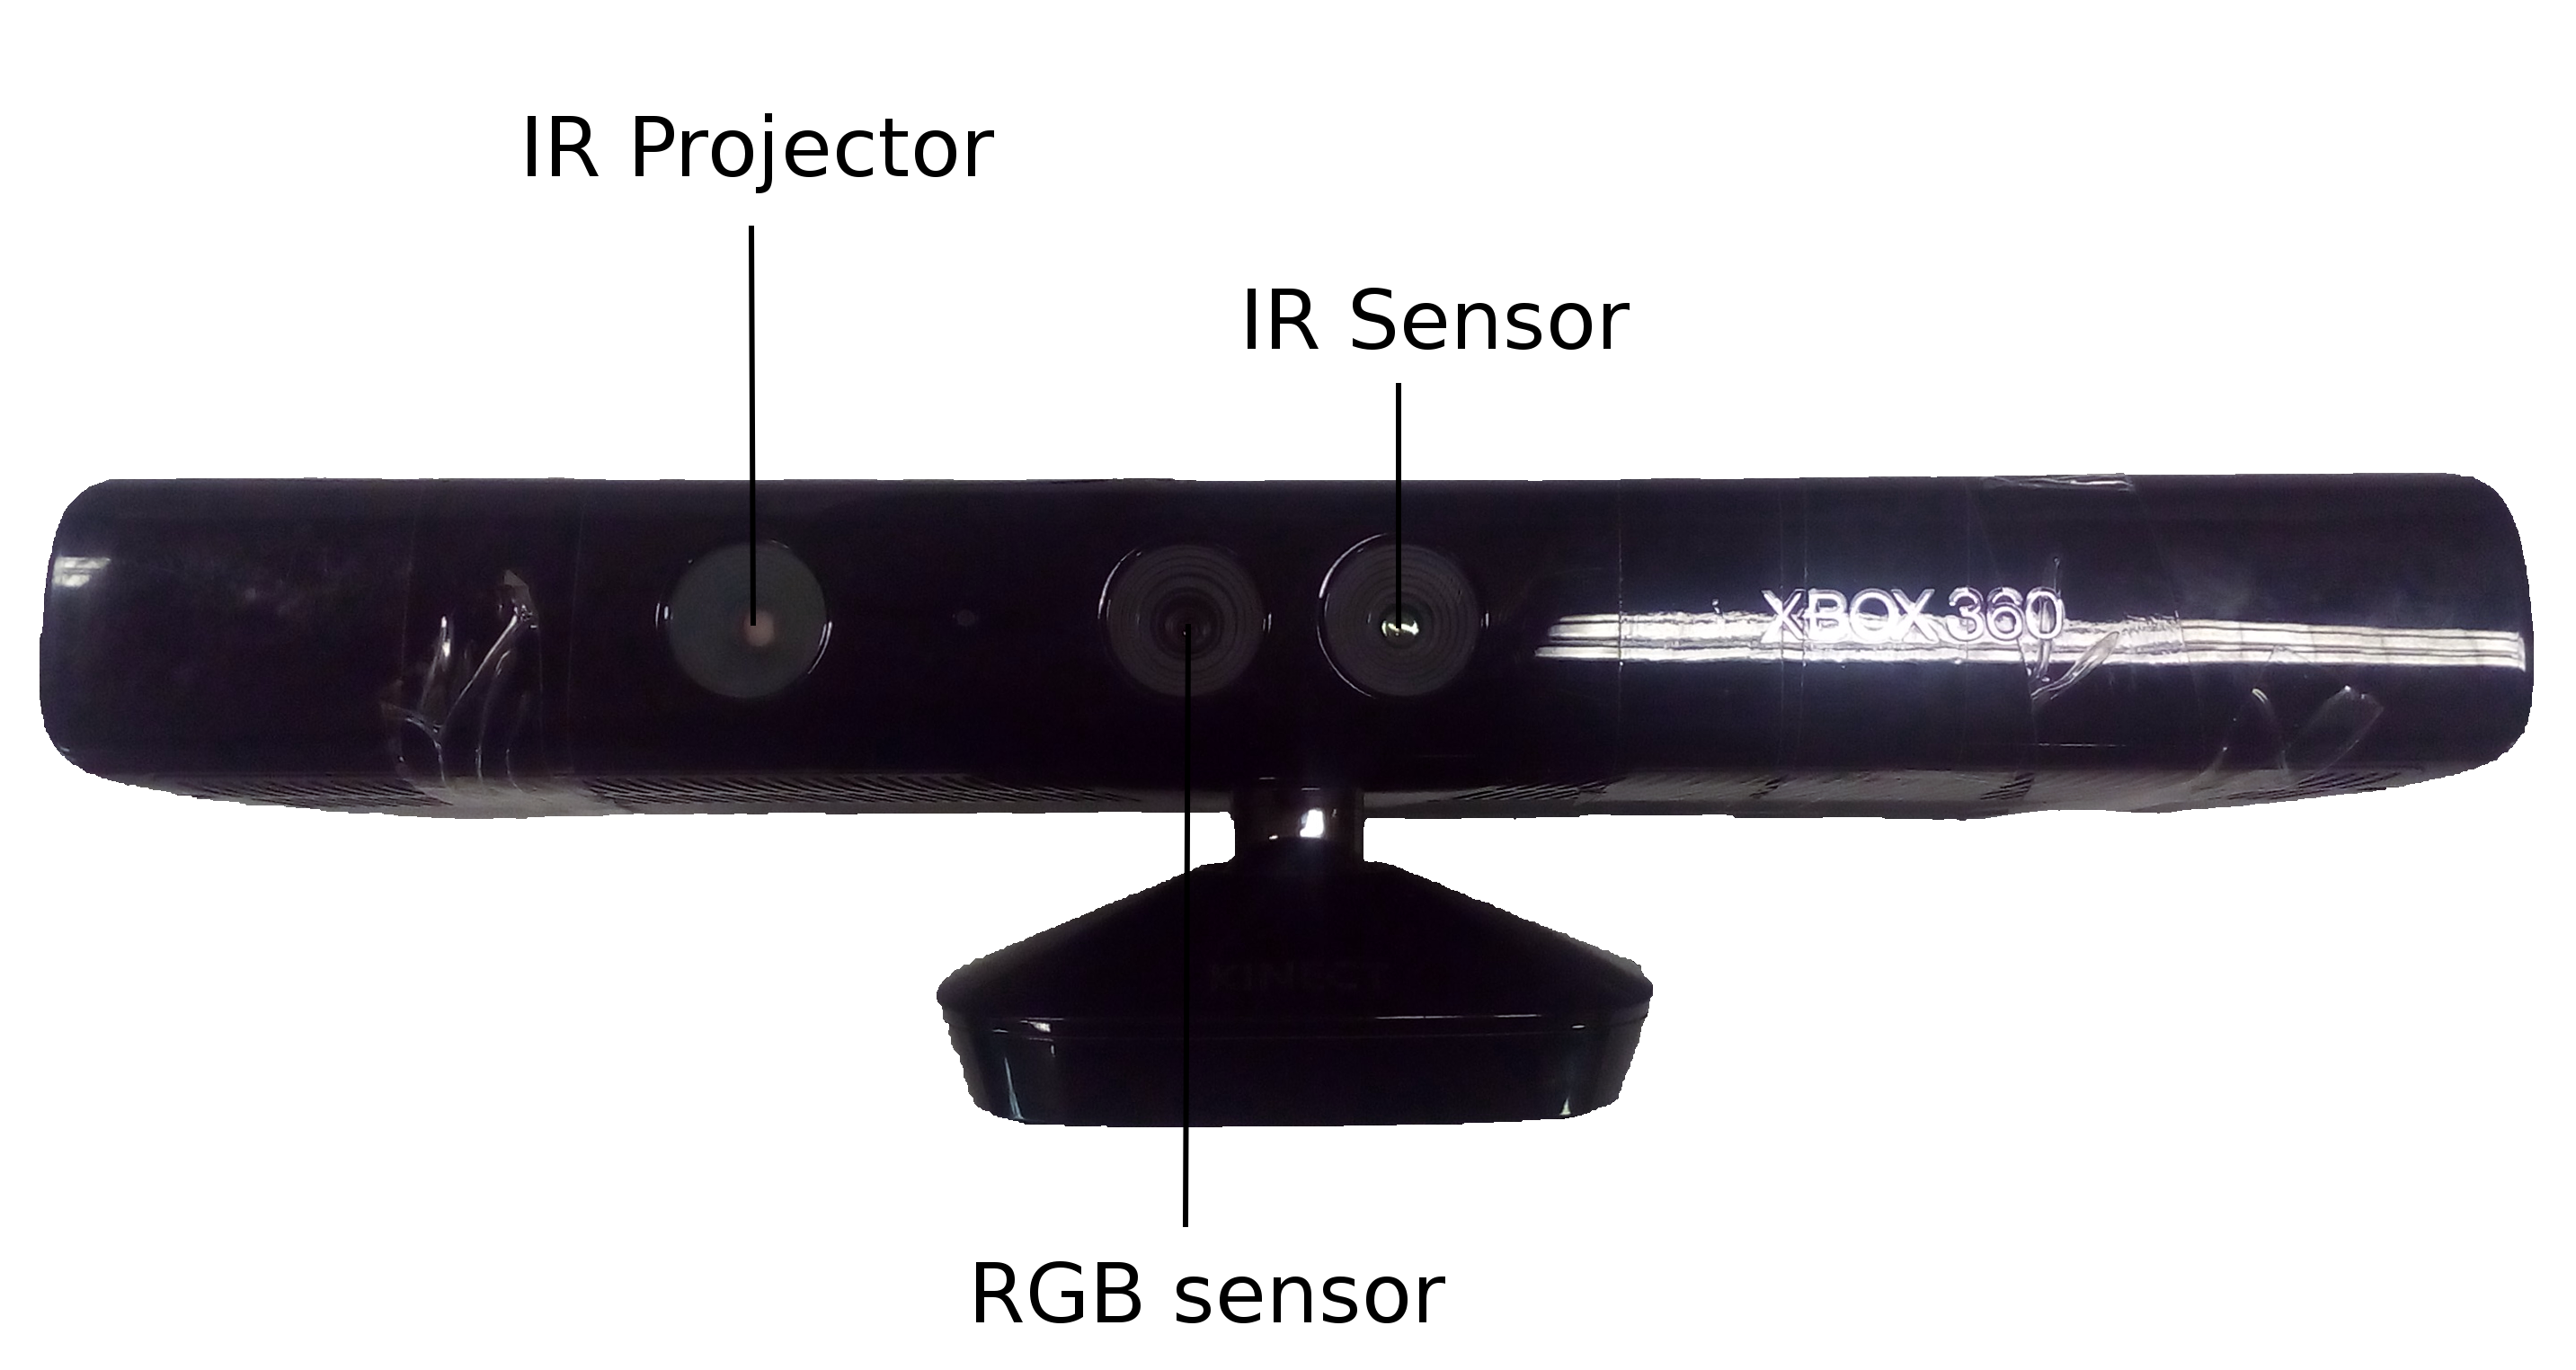
\includegraphics[width=3in]{./Graphics/kinect}
\caption{Microsoft Kinect depth camera, including infrared structured light
projector and sensor, and an RGB camera.\label{fig:kinect}}
\end{figure}

\subsection{Structured light sensors}
In this section, a common type of depth sensor is introduced, which is the one
implemented by Kinect's Primesense hardware, called \emph{structured light
sensor}. This technology was first patented by Shpunt et al. in
\cite{primesense-patent}; although it is used into Microsoft Kinect for its
XBox360 devices, and thus is a mainstream, common device, very few technical
details about the implementation are available. \cite{how-kinect-work}, together
with the original patent's text, remain the best available sources of
information about this kind of technology.

The idea behind structured light sensors is the use of a strong infrared projector
which can draw a known pattern onto the scene. Being made of infrared light,
the pattern will not disturb any RGB camera which is operating in parallel with
it. Primesense devices' projection, in particular, consist in a coherent beam
forming a speckle pattern, as the one shown
in fig.\ref{fig:primesense-speckle}. When the pattern is projected at a certain
depth, it is distorted by the environment, and its reflected image is sampled
by an infrared sensor (acting like a normal camera), put behind an infrared
filter operating with a narrow frequency range in order to remove noise. All of
the processing described into this section is presented here as a serie of
algorithms, but is in fact implemented in hardware within the Primesense's
processing circuitry. This makes it possible to directly get the depth image in
output, with an extremely good framerate ($30\unit{fps}$ for VGA images).

\begin{figure}[htbp]
\centering
\begin{tabular}{c|c}
  \adjustbox{valign=m}{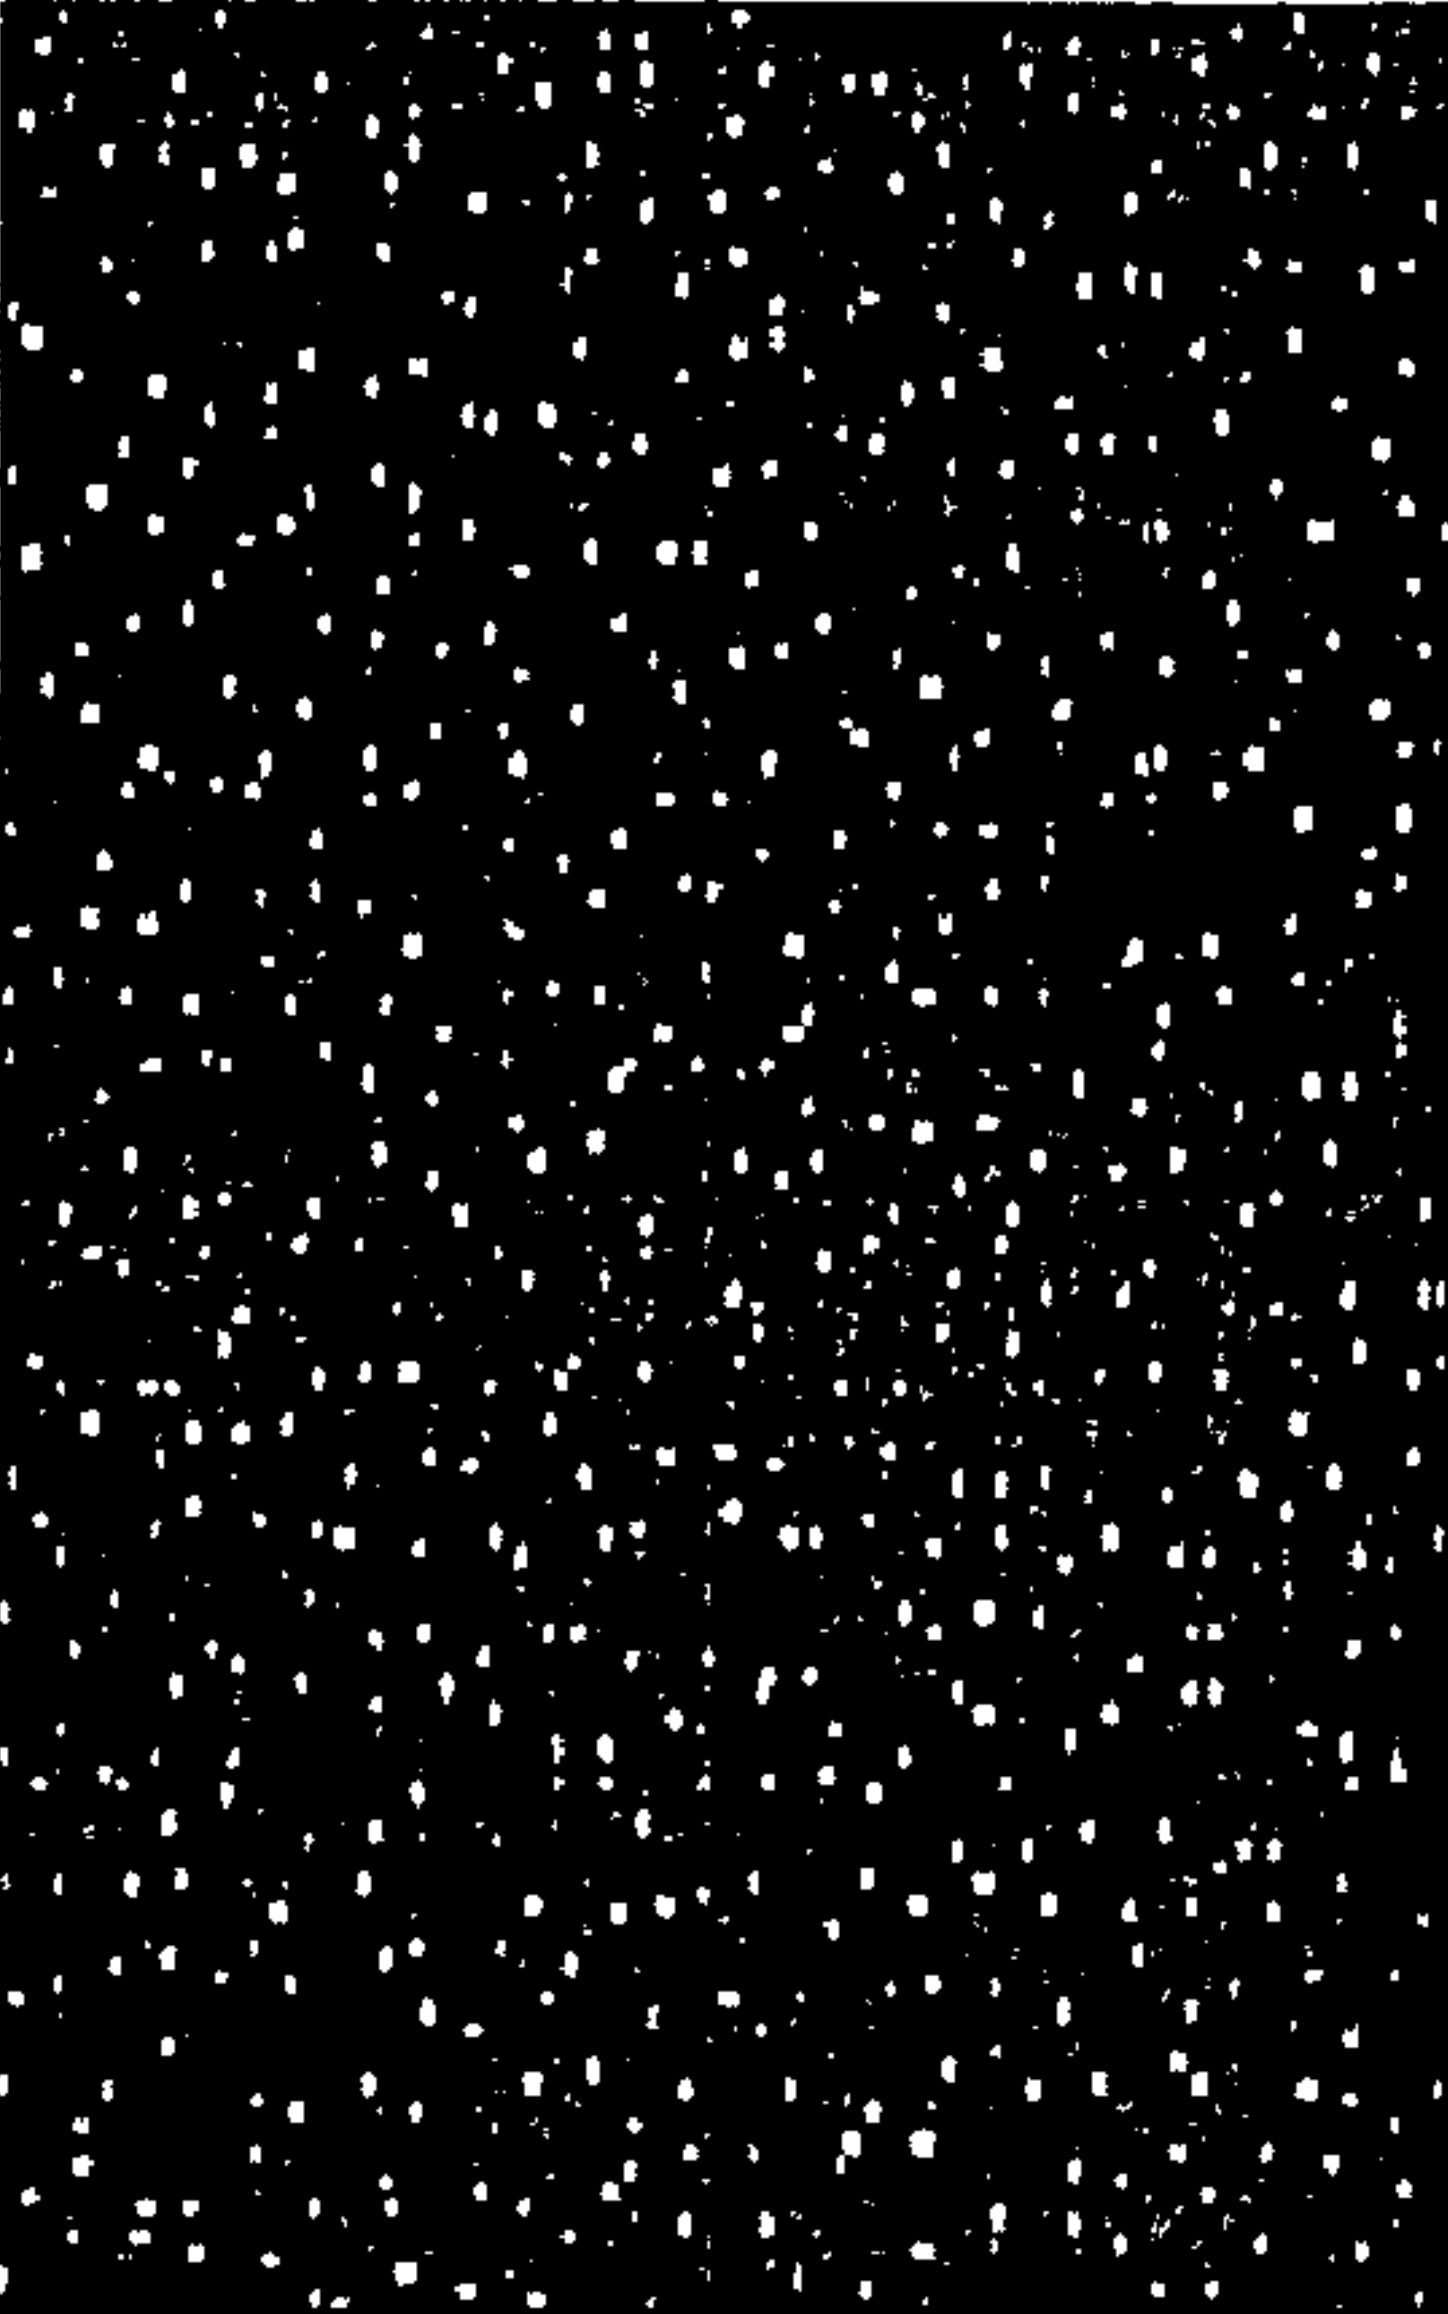
\includegraphics[height=3in]{./Graphics/primesense-speckle}}
&
  \adjustbox{valign=m}{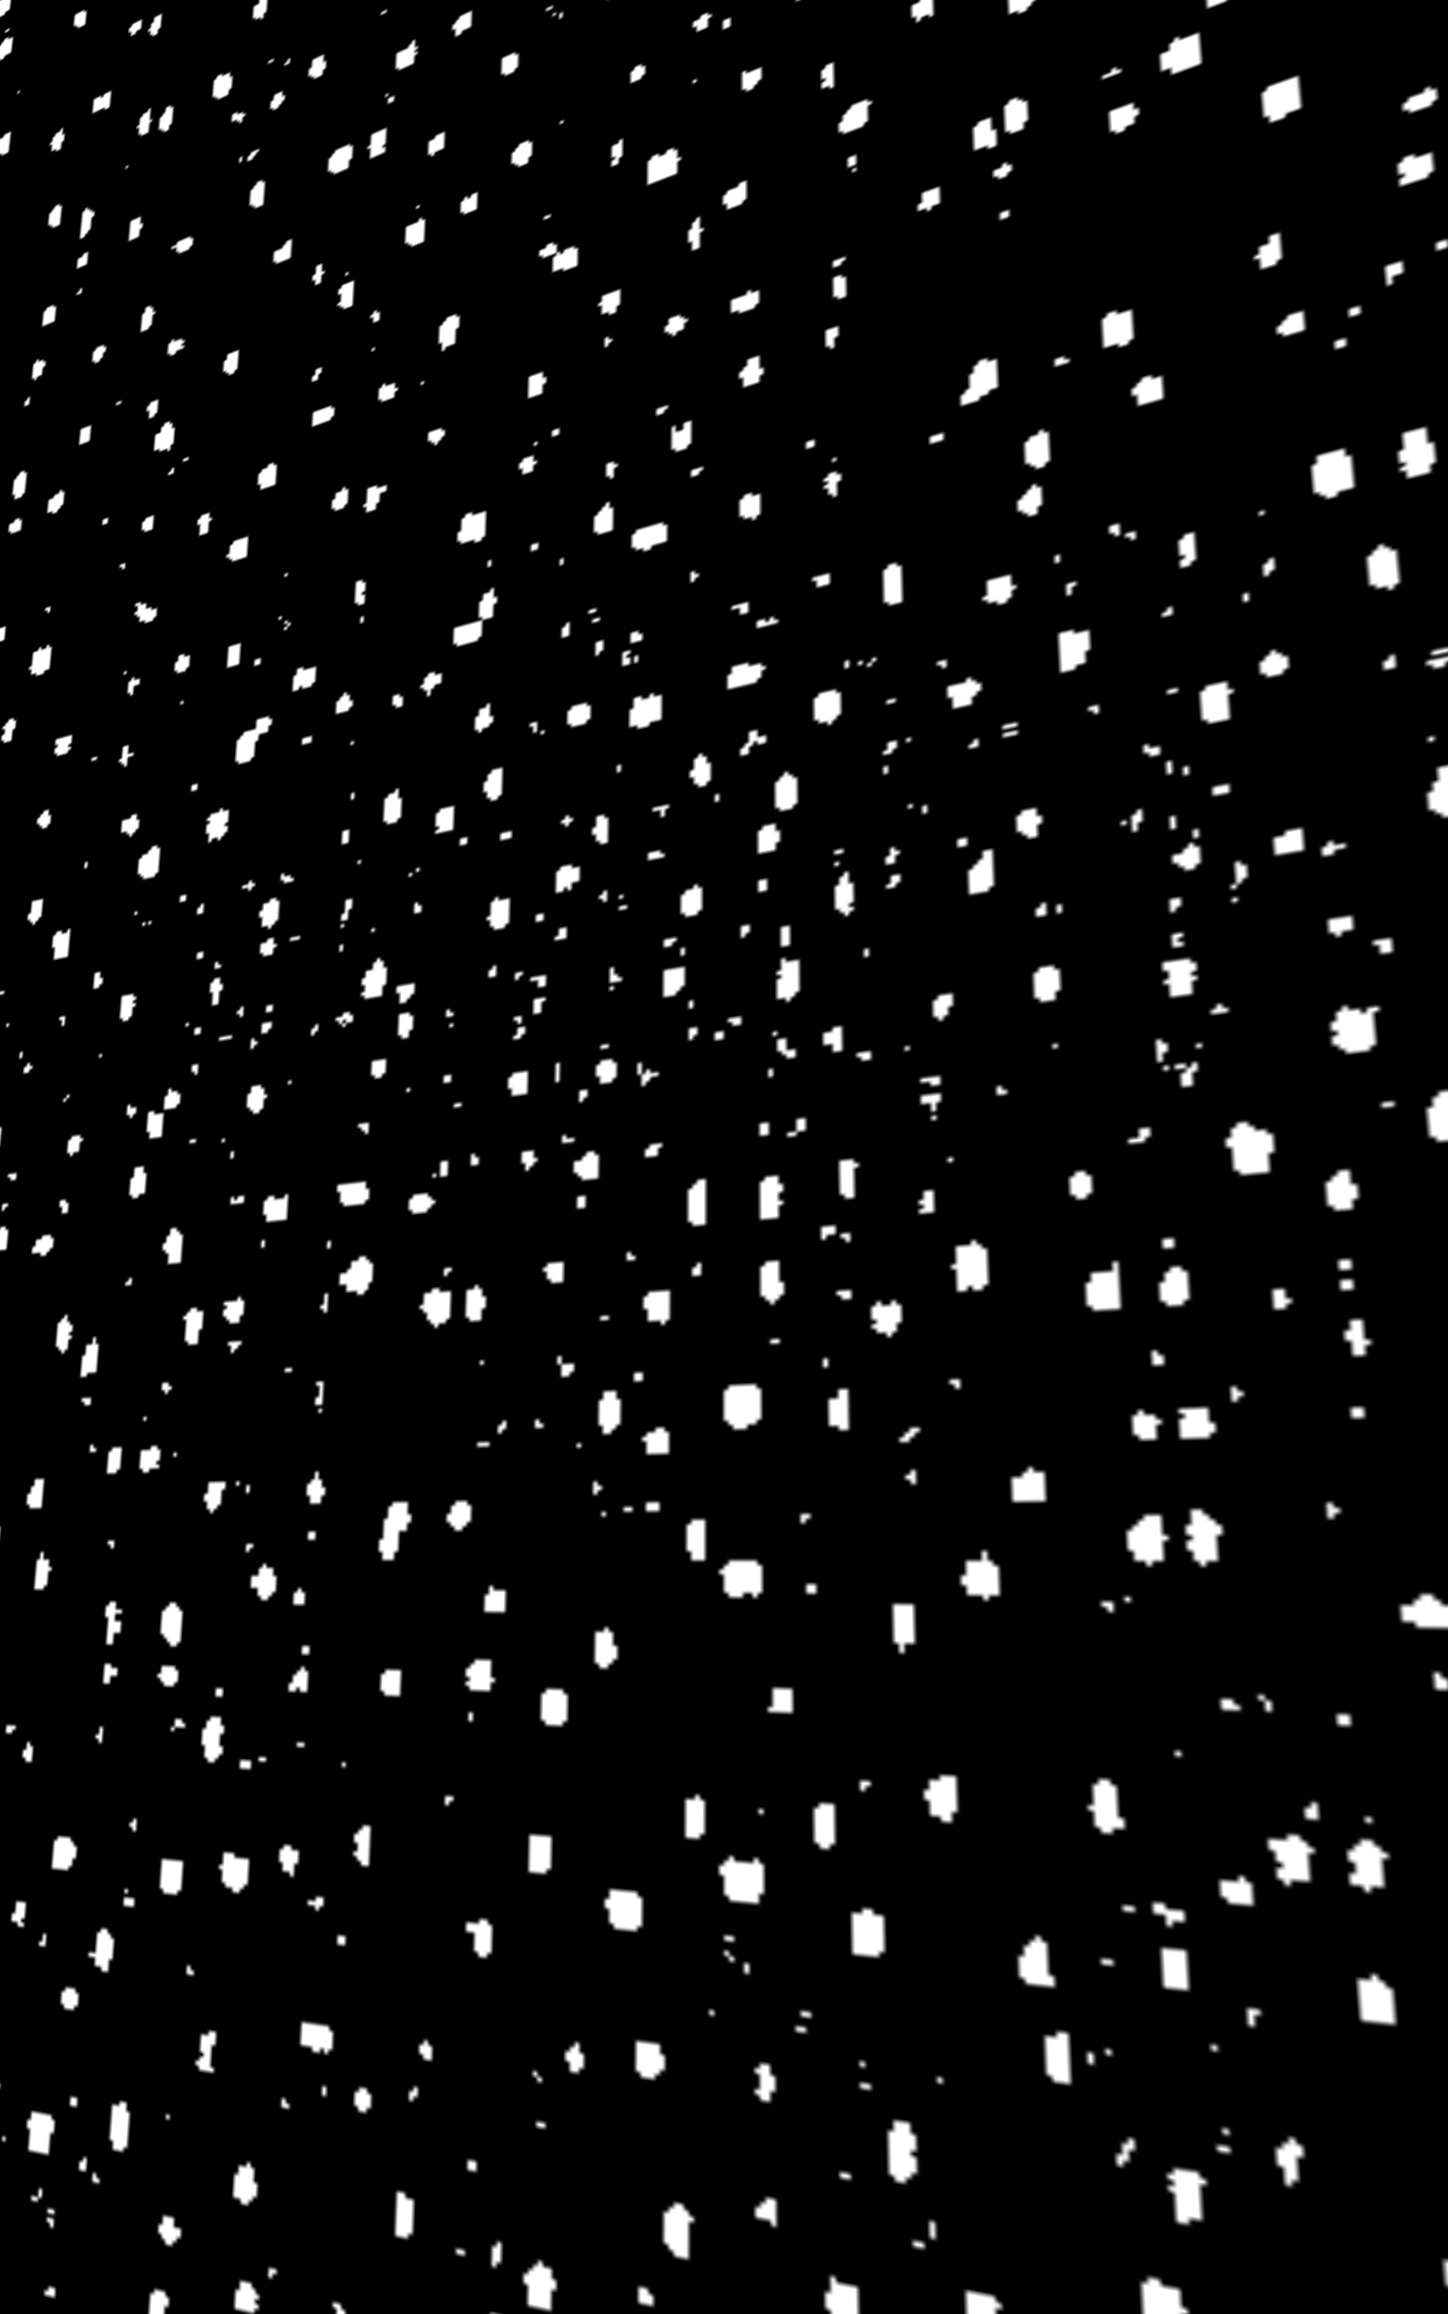
\includegraphics[height=3in]{./Graphics/primesense-speckle-dist}}
\end{tabular}
\caption{Left: speckle pattern, as projected by a Primesense device (from
\cite{primesense-patent}). Right: the same projected pattern, as seen by the
infrared sensor, shows distortion of the pattern depending on the depth of reflection
point.\label{fig:primesense-speckle}}
\end{figure}

Two main techniques are used to obtain a depth value from the sensed infrared
image: \emph{depth from focus}, and \emph{depth from stereo}.

The first one is based on two observations regarding the single spots
composing the pattern: first, as the pattern is both projected
and recaptured using fixed-focus lenses, it will become blurrier the more
distant the reflection point is. Also, lenses used by the capturing device (the
IR sensor) are built in order to have very different focal lengths $f_x$ and
$f_y$ (this concept is explained, together with camera modelling, in sec.
\ref{sec:intrinsics}): they are \emph{astigmatic} lenses. Also, its axes are not
perfectly aligned to the pattern's reference system; in practice, deformation in
the image is introduced by purpose. Usage of astigmatic lenses means that, given
a certain point at a certain depth $d$, it will be more in focus on one principal
axis with respect to the other. The result is that, if a circle of the speckle
is captured using this lens, it will look like an ellipse due to different
blurring on both its directions. The main ellipse's axis angles will vary in function
of $d$.

The second technique used for depth reconstruction is based on the same
principle of stereoscopic vision: as it can be seen in fig.
\ref{fig:kinect}, the projector and the IR sensor are by purpose mounted
at a quite high distance. The result is that each pattern's point is shifted on
one side of the captured image depending on its reflecting distance (i.e. depth
value). Measurement of this shift can improve the results obtained with the
\emph{depth from focus} technique. In fact, this is equivalent to using two
cameras together, in parallel with the depth sensor; the other camera is a
virtual one, as it doesn't match a real sensor: as the pattern image is fixed,
it can be thought of by applying normal stereoscopic matching algorithms with
the captured image and the orthographic drawing of the pattern. This last image
will correspond (for any depth) to the image that would be captured by a camera
placed in correspondence of the projector. With this in mind, stereoscopic
vision can be emulated with a single camera. 
Two advantages are there, with respect to binocular systems: first, no
geometrical calibration is required. Calibration of the sensors' position can be
done once at the factory of origin, and after this it will not suffer from
carriage or system reimplementation, as the sensors are embedded into one single
device. Also and most important, having a fixed pattern to detect extremely
simplifies the problem of features' matching. Features' positions can be
precomputed, and being mainly circular, they are easy to detect in the dynamic
image grabbed by the IR sensor. Knowing their fixed position, triangulation is
almost immediate too.

By combining these two techniques depth can be refined accurately for each
pixel. Most importantly, outliers can be totally filtered out as they will
correspond to very different outputs coming from the first and the second
algorithm; this is a good improvement over binocular systems.

After getting a good point map, the camera model of sec.
\ref{sec:camera_modelling} is used by the camera's hardware to associate to each
obtained spatial location a point into the RGB image taken by the colour sensor.
Again, this procedure is highly simplified by the fact that the relative
position between the two sensors is known a priori. The result of this operation
is what is called a \emph{registered RGBD image}, i.e. an image with four
channels, representing red, green, blue, and depth components of each pixel.

Simplification of the algorithms due to the fixed pattern is the main idea that
allows an efficient implementation of these in hardware; structured light systems are thus
naturally suitable for high frame rates, low cost, high precision depth
measurement solutions.
